% Preamble
\documentclass[11pt]{article}

% Packages
\usepackage{amsmath}
\usepackage[a4paper, margin=0.5in]{geometry}
\usepackage{graphicx} % daj an 1in jak chcesz normalniejszy margines, ale kod mi się w linii nie mieści :P
\usepackage[utf8]{inputenc}
\usepackage[T1]{fontenc}
\usepackage[polish]{babel}
\usepackage{float}
\usepackage{hyperref}

\title{Zadanie 1. Heurystyki konstrukcyjne}
\author{Oskar Kiliańczyk 151863 \& Wojciech Kot 151876}
\date{}

% Document
\begin{document}

\maketitle
\newpage

\section{Opis zadania}\label{sec:opis-zadania}

Podczas zajęć rozważamy zmodyfikowany problem komiwojażera.
Początkowo, obliczamy macierz odległości pomiędzy danymi miastami.
Obliczona macierz odległości między wierzchołkami grafu będzie podstawą dla każdego algorytmu,
a celem jest wyznaczenie dwóch rozłącznych zamkniętych ścieżek (cykli), z których każda zawiera 50\% wierzchołków.
Jeśli liczba wierzchołków jest nieparzysta, jedna ścieżka zawiera jeden wierzchołek więcej.
Kryterium optymalizacji jest minimalizacja łącznej długości obu cykli.

Rozważane instancje problemu pochodzą z biblioteki TSPLib, a są to kroa200 oraz krob200.
Są to instancje dwuwymiarowe euklidesowe, w których każdemu wierzchołkowi przypisane są współrzędne na płaszczyźnie.
Odległość między wierzchołkami liczona jest jako odległość euklidesowa, zaokrąglana do najbliższej liczby całkowitej.
W implementacji algorytmów wykorzystywana będzie wyłącznie macierz odległości, co zapewnia możliwość zastosowania kodu do innych instancji problemu.

\section{Zaimplementowane algorytmy}\label{sec:zaimplementowane-algorytmy}

\subsection{Algorytm zachłanny - metoda najbliższego sąsiada}\label{subsec:algorytm-zachanny---metoda-najblizszego-sasiada}

Algorytm ten wykorzystuje funkcję znajdującą najbliższego sąsiada dla danego wierzchołka (miasta)
Działa ona w następujący sposób: \\
dla każdego miasta, sprawdza czy zostało już odwiedzone \\
jeśli nie, to sprawdza czy dystans jest mniejszy od dystansu z danego miasta do obecnie zapamiętanego jako najbliższe \\
jeśli jest bliższe niż obecnie pamiętane jako najbliższe, zapamiętuje je jako najbliższe \\
jeśli nie ma żadnego miasta obecnie pamiętanego jako najbliższe, przypisuje to miasto \\

Główny algorytm natomiast, wygląda następująco:

\begin{enumerate}
    \item Przydziela wierzchołki startowe do cykli pierwszego i drugiego.
    \item Tworzy tablicę indeksów miast, zaznaczając wszystkie poza startowymi jako nieodwiedzone.
    \item Dopóki istnieją jakieś nieodwiedzone miasta, powtarza następujące kroki:
    \begin{itemize}
        \item Znajduje najbliższego nieodwiedzonego sąsiada do ostatniego wierzchołka cyklu 1.
        \item Dodaje go do cyklu 1 oraz zapisuje w tablicy jako odwiedzony.
        \item Znajduje najbliższego nieodwiedzonego sąsiada do ostatniego wierzchołka cyklu 2.
        \item Dodaje go do cyklu 2 oraz zapisuje w tablicy jako odwiedzony.
    \end{itemize}
    \item Kiedy już nie ma żadnych nieodwiedzonych miast, dopisuje na koniec cykli ich wierzchołki startowe.
    \item Zwraca oba cykle jako znalezione ścieżki.
\end{enumerate}


\subsection{Algorytm zachłanny - metoda rozbudowy cyklu}\label{subsec:algorytm-zachanny---metoda-rozbudowy-cyklu}

Algorytm ten korzysta z funkcji znajdywania najlepszego wstawienia, a działa ona w następujący sposób:

\begin{enumerate}
    \item Przyjmuje jako argumenty:
    \begin{itemize}
        \item obecny cykl,
        \item macierz dystansów,
        \item tablicę indeksów odwiedzonych miast.
    \end{itemize}
    \item Tworzy listę możliwości (nieodwiedzonych wierzchołków).
    \item Ustawia najtańszy koszt na maksymalnie dużą wartość.
    \item Dla każdej możliwości z listy możliwości:
    \begin{enumerate}
        \item Dla każdego możliwego wstawienia w cykl:
        \begin{itemize}
            \item Oblicza wzrost dystansu, jaki spowoduje wstawienie (a więc przy wstawianiu między \(a\) i \(b\) wierzchołka \(c\), oblicza dystans \(|ac| + |bc| - |ab|\)).
            \item Zapisuje najmniejszy znaleziony wzrost dystansu oraz miejsce jego wstawienia.
        \end{itemize}
        \item Jeśli koszt wstawienia obecnie znalezionego wierzchołka jest mniejszy niż obecnie pamiętany najtańszy koszt wstawienia:
        \begin{itemize}
            \item Zapisuje ten koszt jako obecnie najtańszy.
            \item Zapisuje wierzchołek oraz miejsce jego wstawienia.
        \end{itemize}
    \end{enumerate}
    \item Po przejrzeniu wszystkich możliwości zwraca parę \(\langle\)wierzchołek, miejsce wstawienia\(\rangle\).
    \item Dwukrotnie przydziela wierzchołki startowe do cykli pierwszego i drugiego jako początek i koniec cyklu.
    \item Tworzy tablicę indeksów miast, zaznaczając wszystkie poza startowymi jako nieodwiedzone.
    \item Dopóki istnieją jakieś nieodwiedzone miasta, powtarza następujące kroki:
    \begin{enumerate}
        \item Znajduje najtańsze wstawienie, czyli parę \(\langle\)wierzchołek, miejsce w cyklu\(\rangle\) dla cyklu 1.
        \item Wstawia w odpowiednie miejsce cyklu 1 znaleziony wierzchołek.
        \item Zapisuje wierzchołek jako już odwiedzony.
        \item Znajduje najtańsze wstawienie dla cyklu 2.
        \item Jeśli ono nie istnieje (np. bo ostatni wierzchołek został już wstawiony), to kończy pętlę.
        \item Wstawia w odpowiednie miejsce cyklu 2 znaleziony wierzchołek.
        \item Zapisuje wierzchołek jako już odwiedzony.
    \end{enumerate}
    \item Kiedy już nie ma żadnych nieodwiedzonych miast, zwraca oba cykle jako znalezione ścieżki.
\end{enumerate}

Sam algorytm:
\begin{enumerate}
    \item Dwukrotnie przydziela wierzchołki startowe do cykli pierwszego i drugiego jako początek i koniec cyklu.
    \item Tworzy tablicę indeksów miast, zaznaczając wszystkie poza startowymi jako nieodwiedzone.
    \item Dopóki istnieją jakieś nieodwiedzone miasta, powtarza następujące kroki:
    \begin{enumerate}
        \item Znajduje najtańsze wstawienie, czyli parę \(\langle\)wierzchołek, miejsce w cyklu\(\rangle\) dla cyklu 1.
        \item Wstawia w odpowiednie miejsce cyklu 1 znaleziony wierzchołek.
        \item Zapisuje wierzchołek jako już odwiedzony.
        \item Znajduje najtańsze wstawienie dla cyklu 2.
        \item Jeśli ono nie istnieje (np. bo ostatni wierzchołek został już wstawiony), to kończy pętlę.
        \item Wstawia w odpowiednie miejsce cyklu 2 znaleziony wierzchołek.
        \item Zapisuje wierzchołek jako już odwiedzony.
    \end{enumerate}
    \item Kiedy już nie ma żadnych nieodwiedzonych miast, zwraca oba cykle jako znalezione ścieżki.
\end{enumerate}


\subsection{Algorytm z żalem - metoda rozbudowy cyklu}\label{subsec:algorytm-z-zalem---metoda-rozbudowy-cyklu}

\begin{enumerate}
    \item Dwukrotnie przydziela wierzchołki startowe do cykli pierwszego i drugiego jako początek i koniec cyklu.
    \item Tworzy tablicę indeksów miast, zaznaczając wszystkie poza startowymi jako nieodwiedzone.
    \item Dopóki istnieją jakieś nieodwiedzone miasta, powtarza następujące kroki:
    \begin{enumerate}
        \item Dla każdego cyklu:
        \begin{enumerate}
            \item Oblicz koszt rozbudowy cyklu o każde możliwe nieodwiedzone dotąd miasto dla każdego możliwego punktu rozbudowy cyklu.
            \item Posortuj listę kosztów (rosnąco).
            \item Oblicz dwużal jako różnicę pomiędzy drugim najlepszym a najlepszym wynikiem z listy kosztów.
            \item Jeżeli wyliczony żal jest większy niż dla jakiegokolwiek innego wstawienia miasta, to uznaj go za najlepszy.
        \end{enumerate}
        \item Rozszerz cykl w miejscu wskazanym dla najlepszego wyliczonego dwużalu.
        \item Zapisz wierzchołek jako już odwiedzony.
    \end{enumerate}
    \item Kiedy już nie ma żadnych nieodwiedzonych miast, zwraca oba cykle jako znalezione ścieżki.
\end{enumerate}


\subsection{Algorytm z żalem - metoda rozbudowy cyklu z żalem ważonym}\label{subsec:algorytm-z-zalem---metoda-rozbudowy-cyklu-z-zalem-wazonym}

\begin{enumerate}
    \item Dwukrotnie przydziela wierzchołki startowe do cykli pierwszego i drugiego jako początek i koniec cyklu.
    \item Tworzy tablicę indeksów miast, zaznaczając wszystkie poza startowymi jako nieodwiedzone.
    \item Dopóki istnieją jakieś nieodwiedzone miasta, powtarza następujące kroki:
    \begin{enumerate}
        \item Dla każdego cyklu:
        \begin{enumerate}
            \item Oblicz koszt rozbudowy cyklu o każde możliwe nieodwiedzone dotąd miasto dla każdego możliwego punktu rozbudowy cyklu.
            \item Posortuj listę kosztów (rosnąco).
            \item Oblicz dwużal ważony jako różnicę pomiędzy drugim najlepszym a najlepszym wynikiem z listy kosztów z odpowiednimi wagami (domyślnie $waga_2 = (-1) \cdot waga_1$).
            \item Jeżeli wyliczony żal jest większy niż dla jakiegokolwiek innego wstawienia miasta, to uznaj go za najlepszy.
        \end{enumerate}
        \item Rozszerz cykl w miejscu wskazanym dla najlepszego wyliczonego dwużalu.
        \item Zapisz wierzchołek jako już odwiedzony.
    \end{enumerate}
    \item Kiedy już nie ma żadnych nieodwiedzonych miast, zwraca oba cykle jako znalezione ścieżki.
\end{enumerate}

\subsection{Własny jakiś dziki algorytm, jak nam się będzie chciało, bo imo bym zrobił coś}

\begin{verbatim}
    kodkodkod
\end{verbatim}


\section{Wyniki eksperymentu obliczeniowego}\label{sec:wyniki-eksperymenty-obliczeniowego}

\subsection{Algorytm zachłanny - metoda najbliższego sąsiada}\label{subsec:algorytm-zachanny---metoda-najblizszego-sasiada2}

Graficzną reprezentację wyników dla algorytmu zachłannego metodą najbliższego sąsiada przestawiono na~\ref{fig:Greedy-nearest-kroA, fig:Greedy-nearest-kroB}
\begin{figure}[H]
    \centering
    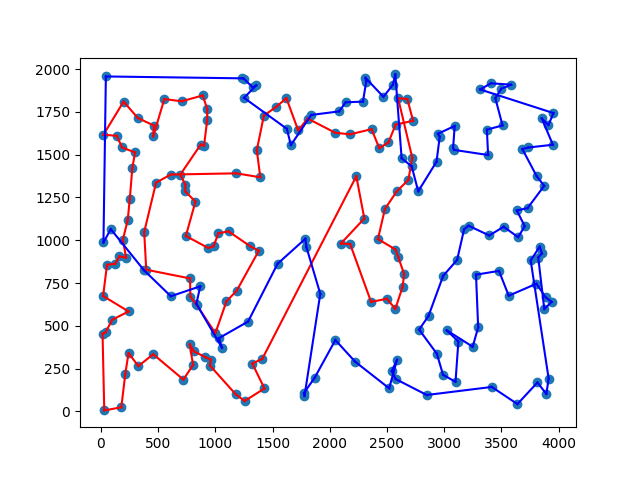
\includegraphics{best_paths/greedy_nearest_neighbor_kroA200.tsp.png}
    \caption{Instancja kroA200}
    \label{fig:Greedy-nearest-kroA}
\end{figure}
\begin{figure}[H]
    \centering
    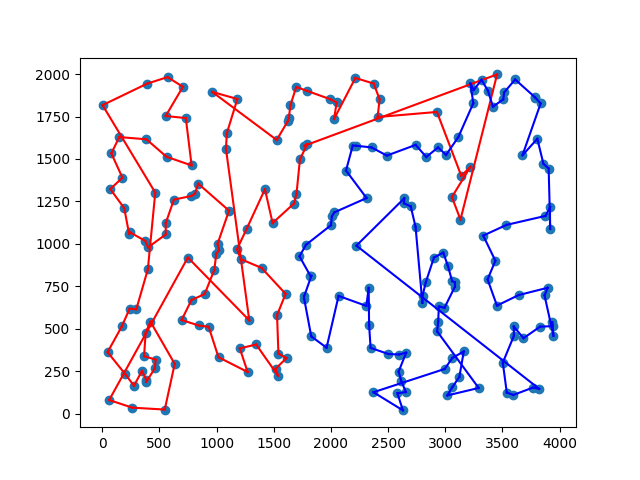
\includegraphics{best_paths/greedy_nearest_neighbor_kroB200.tsp.png}
    \caption{Instancja kroB200}
    \label{fig:Greedy-nearest-kroB}
\end{figure}


\subsection{Algorytm zachłanny - metoda rozbudowy cyklu}\label{subsec:algorytm-zachanny---metoda-rozbudowy-cyklu2}

Graficzną reprezentację wyników dla algorytmu zachłannego metodą rozbudowy cyklu przestawiono na~\ref{fig:Greedy-cycle-kroA, fig:Greedy-cycle-kroB}
\begin{figure}[H]
    \centering
    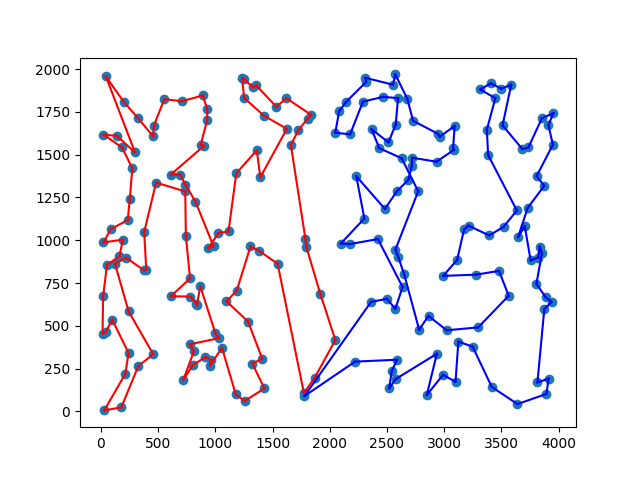
\includegraphics{best_paths/greedy_cheapest_insertion_kroA200.tsp.png}
    \caption{Instancja kroA200}
    \label{fig:Greedy-cycle-kroA}
\end{figure}
\begin{figure}[H]
    \centering
    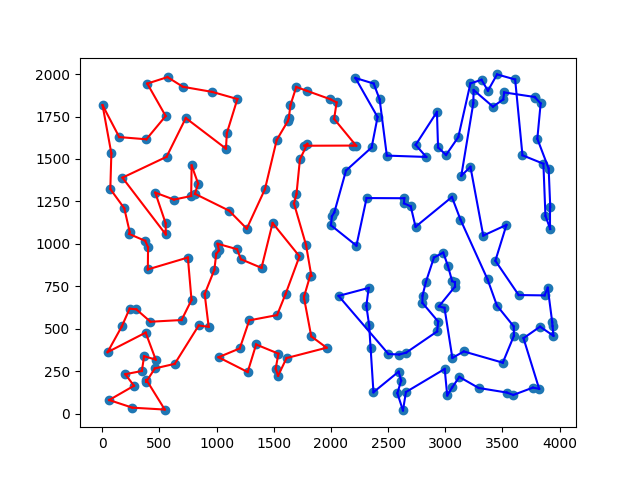
\includegraphics{best_paths/greedy_cheapest_insertion_kroB200.tsp.png}
    \caption{Instancja kroB200}
    \label{fig:Greedy-cycle-kroB}
\end{figure}

\subsection{Algorytm dwużal}\label{subsec:algorytm-dwużal}
Graficzną reprezentację wyników dla algorytmu dwużalu przestawiono na~\ref{fig:Two-regret-kroA, fig:Two-regret-kroB}
\begin{figure}[H]
    \centering
    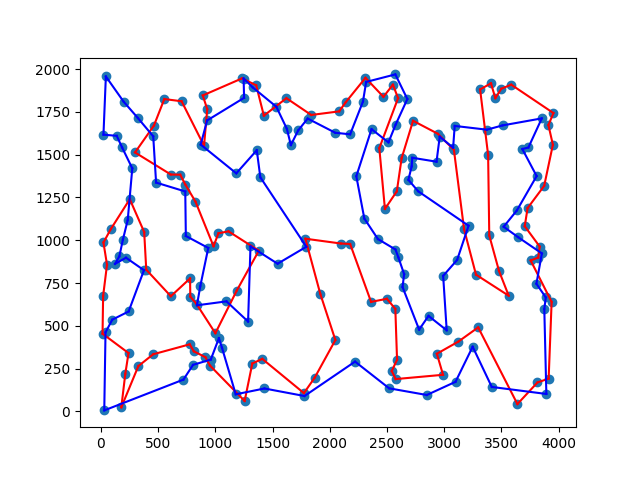
\includegraphics{best_paths/two_regret_kroA200.tsp.png}
    \caption{Instancja kroA200}
    \label{fig:Two-regret-kroA}
\end{figure}
\begin{figure}[H]
    \centering
    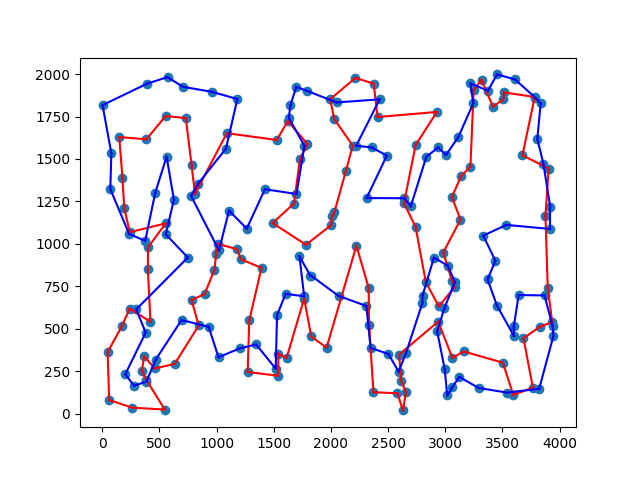
\includegraphics{best_paths/two_regret_kroB200.tsp.png}
    \caption{Instancja kroB200}
    \label{fig:Two-regret-kroB}
\end{figure}

\subsection{Algorytm dwużal ważony}\label{subsec:algorytm-dwużal-ważony}
Graficzną reprezentację wyników dla algorytmu dwużalu ważonego przestawiono na~\ref{fig:Two-regret-weighted-kroA, fig:Two-regret-weighted-kroB}
\begin{figure}[H]
    \centering
    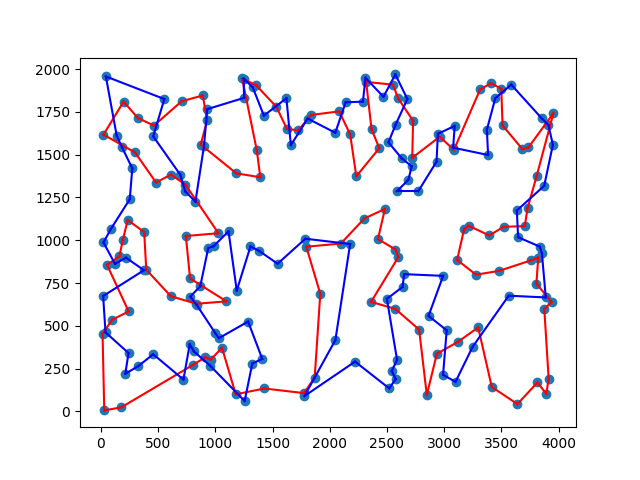
\includegraphics{best_paths/weighted_two_regret_kroA200.tsp.png}
    \caption{Instancja kroA200}
    \label{fig:Two-regret-weighted-kroA}
\end{figure}
\begin{figure}[H]
    \centering
    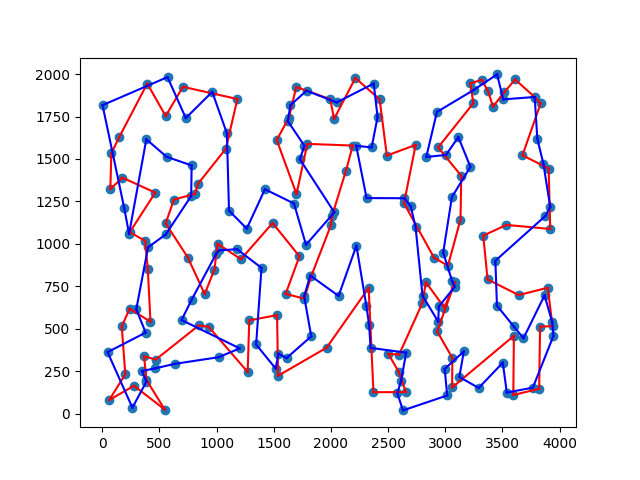
\includegraphics{best_paths/weighted_two_regret_kroB200.tsp.png}
    \caption{Instancja kroB200}
    \label{fig:Two-regret-weighted-kroB}
\end{figure}

\section{Porównanie algorytmów}\label{sec:porównanie-algorytmów}
\begin{table}[H]
    \centering
    \begin{tabular}{|c||c|c|c||c|c|c|}
        \hline
        Algorytm & \multicolumn{3}{c||}{KroA200.tsp} & \multicolumn{3}{c|}{KroB200.tsp} \\
        \cline{2-4} \cline{5-7}
        & Min & Średnia & Max & Min & Średnia & Max   \\
        \hline
        Nearest Neighbor Greedy & 36755.00 & 42701.26 & 47080.00 & 38121.00 & 42122.12 & 47313.00 \\
        \hline
        Cycle Extension Greedy & 35396.00 & 37966.75 & 41224.00 & 35733.00 & 38455.32 &  39991.00 \\
        \hline
        Two regret & 42450.00 & 44536.57 & 46038.00 & 42029.00 & 43420.64 & 45065.00 \\
        \hline
        Weighted Two regret & 50016.00 & 51307.46 & 53146.00 & 48945.00 & 50277.95 & 52187.00 \\
        \hline
    \end{tabular}
    \label{tab:wyniki-eksperymentu}
    \caption{Wyniki eksperymentu obliczeniowego}
\end{table}

\section{Wnioski}\label{sec:wnioski}

Żal nie działa, chociaż byśmy chcieli, ale żal rozwiązuje zwykły TSP.
Może w połączeniu z algorytmem klastrującym, jakimś k-means zadziałałby lepiej, ale strasznie krzywdzące dla niego jest też to że ścieżki MUSZĄ być równej długości

\section{Link do repo}\label{sec:link-do-repo}
Kod źródłowy w repozytorium GitHub dostępny pod linkiem: \\
\href{https://github.com/KotZPolibudy/PUT_IMO/tree/main/TSP_heuristic}{Repozytorium TSP Heuristics}.

\end{document}
